% !TeX encoding = UTF-8
% !TeX spellcheck = fr_FR
% !TeX root = ../mythesis.tex
% !TeX program = pdflatex (build)
%%% TeXmaker : no 'magic comments' but set Root with Options > Set as master file

%useful stuff for what follows
\newcommand{\kperp}{\mathbf{k}_\perp}
\newcommand{\rperp}{\mathbf{r}_\perp}
\newcommand{\Ehat}{\hat{\mathcal{E}}}
\newcommand{\dEhat}{\delta\hat{\mathcal{E}}}
\newcommand{\ak}{\hat{a}_{\mathbf{k}_\perp}}
\newcommand{\akdag}{\hat{a}^\dagger_{\mathbf{k}_\perp}}
\newcommand{\amk}{\hat{a}_{-\mathbf{k}_\perp}}
\newcommand{\amkdag}{\hat{a}^\dagger_{-\mathbf{k}_\perp}}
\newcommand{\bk}{\hat{b}_{\mathbf{k}_\perp}}
\newcommand{\bkdag}{\hat{b}^\dagger_{\mathbf{k}_\perp}}
\newcommand{\bmk}{\hat{b}_{-\mathbf{k}_\perp}}
\newcommand{\bmkdag}{\hat{b}^\dagger_{-\mathbf{k}_\perp}}

\graphicspath{{./}{./fig/}{./chap1/fig/}}




\part{Theory of Microcavity Exciton Polaritons}


\chapter{Microcavity Exciton Polaritons}\label{chap:polariton_theory}

Photons are massless particles, yet when confined within an optical cavity, they obtain an effective mass and exhibit a parabolic dispersion relation. However, two photons in the cavity do not interact with each other in the sense that they do not attract or repel each other as massive particles would do.

Whenever an electromagnetic field is shined on a material, the dipoles of the medium oscillate and change the refractive index seen by the field. At high intensity, the change in the refractive index can depend on the square of the electric field, which is then called the Kerr effect. Since a local variation of the refractive index deflects light, a high-intensity region in the material can modify the trajectory of an incoming beam. From this point of view, one can see how photon-photon interaction can arise in a nonlinear medium.

If the medium is chosen such that the resonance frequency of the dipoles matches the resonance of the optical microcavity, the light can be trapped in the sample and experience effective interaction through the medium. When the coupling of the light with the medium is strong enough to exceed the losses of the whole system, one can achieve the strong coupling regime. In this regime, the new eigenstates of the system are the so-called polaritons, which are a superposition of the photon and the dipole excitation of the medium. This hybrid state of matter inherits properties from both photons and matter excitations and forms the constitutive particles of the quantum fluid considered later.

In the present case, the strong coupling regime is achieved in a semiconductor microcavity by inserting two-dimensional quantum wells at the antinode of the electromagnetic field of a high-quality factor optical microcavity. In such devices, polaritons arise from the coupling between the cavity photons and the excitons of the quantum wells.

This chapter is dedicated to describing photons and excitons separately before showing how they couple in the sample to form polaritons. Then, from a microscopic description, one will derive the macroscopic equations of motion of the fluid and find that polaritons can be described in the usual Quantum Fluid framework with a driven dissipative Gross-Pitaevskii equation.

\section{Microcavity Photons}

\begin{figure}[H]
    \centering
    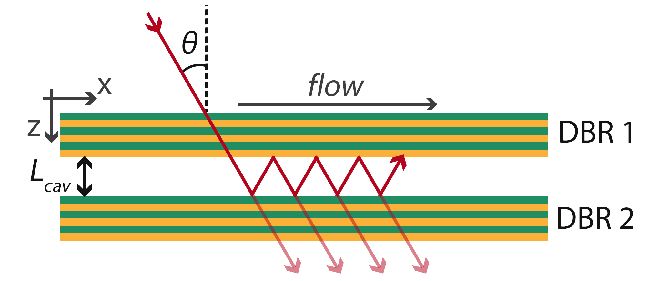
\includegraphics[width=\textwidth]{chap1/fig/cavity_geometry.pdf}
    \caption{Photon in a planar microcavity}
    \label{fig:cavity_geometry}
\end{figure}

\textbf{Planar microcavity parameters:}
First, let us consider an electromagnetic field incident at an angle $\theta$ on a planar microcavity made with two mirrors with reflectivities $R_1$ and $R_2$, separated by a distance $L$. The z-axis is normal to the mirrors as shown in \autoref{fig:cavity_geometry}. The phase shift acquired during a single round trip in the cavity is $\Delta \phi (\theta)=2nk_0L\cos(\theta)$, with $n$ the refractive index of the medium and $k_0=2\pi/\lambda$ the wave vector of the field in vacuum. The interference between the multiple reflections sets the resonance condition of the cavity, and the transmission of the field can be written as:

\begin{equation}
    T(\theta)=\frac{R_1R_2}{1+R_1R_2-\sqrt{R_1R_2}\cos(\Delta \phi(\theta)/2)}
    \label{eq:transmission_theta}
\end{equation}

\noindent From this, one can define the decay rate of the field oscillation known as the quality factor:
\begin{equation}
    Q=\frac{\omega_\gamma}{\Delta \omega_\gamma}
    \label{eq:Q}
\end{equation}
with $\omega_\gamma$ the resonance frequency of the cavity and $\Delta \omega_\gamma$ the linewidth of the resonance, which sets the lifetime of the photon in the cavity through $\tau_\gamma=1/\Delta \omega_\gamma$ and depends on the mirrors' reflectivities. Another important parameter describing the cavity is its frequency resolution, which is encoded in the cavity finesse through:

\begin{equation}
    \mathcal{F}=\pi \frac{\Delta \omega_\gamma}{\delta \omega_\gamma} = \pi \frac{\sqrt{R_1R_2}}{1-R_1R_2}
    \label{eq:F}
\end{equation}

where $\Delta \omega_\gamma$ is the Free Spectral Range (FSR) representing the frequency difference between two successive longitudinal modes of the cavity. To achieve strong coupling with the nonlinear medium, the photon needs to stay trapped in the cavity long enough to interact with the medium. In other words, the quality factor of the cavity must be very high, which means using mirrors with high reflectivities. This can be achieved with Distributed Bragg Reflectors (DBR) mirrors.

\begin{figure}[h]
    \centering
    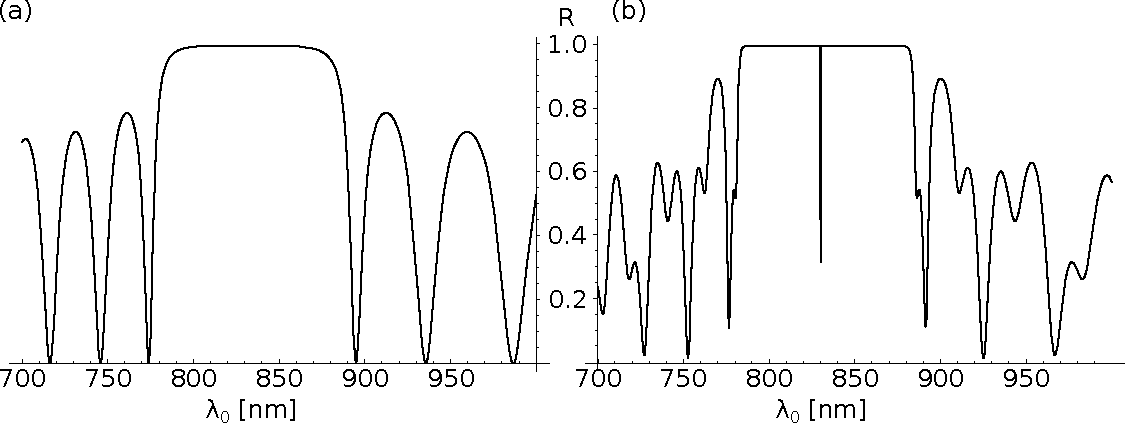
\includegraphics[width=1\linewidth]{chap1/fig/DBR.pdf}
    \caption{\textbf{DBR and Fabry-Perot cavity reflectivity.} \textbf{(a)} Reflectivity $R$ of a Bragg mirror of 20 pairs of Ga$_{0.9}$Al$_{0.1}$As/AlAs, illuminated at normal incidence for different wavelengths $\lambda$. The DBR has a reflectivity close to 1 over a large range of wavelengths called the stop-band, centered on $\lambda_0$ = 836 nm by tuning the thickness of each of the mirror layers. \textbf{(b)} Corresponding reflectivity of the optical cavity built from the facing of two DBR mirrors identical to that in (a) and separated by a distance $L_{\mathrm{cav}} = 2\lambda_0 / n_{\mathrm{cav}}$, leading to the appearance of a very narrow resonance at $\lambda_0$. Adapted from ??.}
    \label{fig:DBR}
\end{figure}

\textbf{Distributed Bragg Reflectors.} These reflectors consist of a series of N alternating layers composed of two materials with different refractive indices $n_1<n_2$. This configuration causes partial reflection of the electromagnetic field at each of the N interfaces, resulting in a very high overall reflection coefficient, $R$, which is expressed as follows:

\begin{equation}
    R = \left[  \dfrac{(n_2/n_1)^{2N} - n_f/n_0}{(n_2/n_1)^{2N} + n_f/n_0} \right]^2,
\end{equation}

with $n_0$ and $n_f$ representing the refractive indices of the media before and after the mirrors. \autoref{fig:DBR} illustrates the evolution of $R$ in relation to the wavelength of the electromagnetic field for one DBR mirror used in our system. This mirror is constructed with 20 pairs of $\text{Ga}_{0.9}\text{Al}_{0.1}\text{As}/\text{AlAs}$ layers, having refractive indices $n_2 = 3.48$ and $n_1 = 2.95$ respectively. The reflection coefficient $R$ is 0.9985 across a broad wavelength range, known as the stop-band, centered around a wavelength of $\lambda_0 = 836$ nm. This central wavelength is achieved by setting the thickness of the layers to $d_{1,2} = \lambda_0 / 4n_{1,2}$. The microcavity used in the experiments is built by facing two of those DBR mirrors separated by a distance $L_{\mathrm{cav}}=3\lambda_0/2n_{\mathrm{cav}}$, giving rise to a very narrow resonance at $\lambda_0$ with three field antinodes within the cavity. The parameters of the cavity are summarized in \autoref{DBR_params}.

\begin{center}
    \begin{tabular}{ |p{1.5cm}|p{1.5cm}|p{1.5cm}|p{1.5cm}|p{1.5cm}|p{1.5cm}|}
    \hline
    \multicolumn{6}{|c|}{Fabry-Perot cavity parameters} \\
    \hline
    \hline
    $R_1$ & $R_2$ & $n_1$ & $n_2$ & $n_{cav}$ & $\lambda_0$ (nm) \\
    \hline
    0.9992  &  0.9985 & 2.95 & 3.48 & 3.54 & 836\\
    \hline
    \label{DBR_params}
    \end{tabular}
\end{center}

With the above-described DBR, the cavity has a finesse $\mathcal{F}=2850$ from which we can infer the photon lifetime:
\begin{equation}
    \delta \omega_{\gamma} = \dfrac{\Delta \omega_{\gamma}}{\mathcal{F}} = \dfrac{c}{n_{\mathrm{cav}} L_{\mathrm{eff}}} \dfrac{1-R}{\sqrt{R}},
\end{equation}
where $L_{\mathrm{eff}}= L_{\mathrm{cav}}+L_{\mathrm{bragg}}$ is the effective length of the sample taking into account the penetration of the field in the mirrors.
\begin{equation}
    L_{\mathrm{Bragg}} = \dfrac{\lambda_0}{2} \dfrac{n_1 n_2}{n_{\mathrm{cav}} (n_2 - n_1)}
\end{equation}
which gives $\tau_{\gamma} = \frac{1}{\delta \omega_{\gamma} }= 5$ ps.

\bigskip\noindent
\textbf{Transverse dynamics of the photon.} The energy of the photon within the sample can be written as:
\begin{equation}
    E_\gamma = \dfrac{\hbar c}{n_{\mathrm{cav}}} \sqrt{k_x^2 + k_y^2 + k_z^2}.
\label{free_space_photon}
\end{equation}
The resonance condition of the cavity fixes the photon wavevector along the z component. 

\begin{equation}
    k_z = \dfrac{2\pi n_{\mathrm{cav}}}{\lambda_0}.
    \label{eq:kz}
\end{equation}
In the paraxial approximation $k_x,k_y \ll k_z$, one can expand \eqref{free_space_photon} in terms of $\frac{||\bm{k_{\parallel}}||}{||\bm{k_z}||}$ as:
\begin{equation}
    E_\gamma = \dfrac{\hbar c}{n_{\mathrm{cav}}} \sqrt{k_z^2 + k_{\parallel}^2} = E_0 \left( 1 + (\hbar k_{\parallel })^2 \dfrac{c ^2}{2(n_{\mathrm{cav}} E_0)^2} \right).
    \label{eq:paraxial_photon}
\end{equation}
where $\bm{k_{\parallel}}=\bm{k_x}+\bm{k_y}$ is the wavevector in the transverse plane and $E_0=hc/\lambda_0$ is the photon energy in free space. We can identify the effective mass of the photon by writing \eqref{eq:paraxial_photon} with the usual form of the kinetic energy of a massive particle:

\begin{equation}
    E_\gamma = E_0 + \dfrac{p_{\parallel}^2}{2m_{\gamma}}  
    \label{eq:photon_mass}
\end{equation}
where we identify $m_{\gamma} = \dfrac{\hbar n_{\mathrm{cav}}^2}{\lambda_0 c}$ which is inversely proportional to the second derivative of the energy with respect to $k_{\parallel}$:

\begin{equation}
    \dfrac{1}{m_{\gamma}} = \dfrac{1}{\hbar^2}\dfrac{\partial^2 E_{\gamma}}{\partial k_{\parallel}^2}
    \label{eq:mass}
\end{equation}

\noindent\textbf{Momentum conservation:}
We mentioned the necessity to have a high quality factor to later achieve strong coupling. One could then ask why do we stick to planar designs, which are generally not the best solution to get a high Q factor since they are known to be unstable except for plane waves. The answer lies in the calculation just above. Indeed, the advantage of having a planar design is the translational invariance in the xy plane, which brings $\bm{k_{\parallel}}$ conservation. As a consequence, if one shines a laser with a given $\bm{k_{\parallel}}$, light will behave in the cavity as a massive particle moving at velocity $v_\gamma=\hbar \bm{k_{\parallel}}/m_\gamma$. In the picture of creating a fluid whose flow is controlled, the planar design then appears as a wise choice.

\bigskip\noindent

\noindent\textbf{A direct link between incidence angle and in plane momentum $k_{\parallel}$:}
As shown in \autoref{fig:cavity_geometry} the incidence angle $\theta= (\theta_x, \theta_y)$ of the incoming field is related to the in-plane momentum $k_{\parallel}$ as :

\begin{equation}
    k_{x} = k_0 \sin(\theta_x) \\
    k_{y} = k_0 \sin(\theta_y)
    \label{eq:kpar}
\end{equation}

Controlling the in plane momentum of photons and latter of polaritons then boils down to control the local incidence angle of the field, in other words, the transverse phase of the incoming beam. This is a crucial point for the experiments as it allows to control the flow of the fluid by changing the laser phase.

\bigskip\noindent
\textbf{Conclusion:}
This section revealed how trapping light in a planar microcavity grants it effective mass and lifetime. The next section will explore the semiconducting media that can be inserted into these cavities, especially the bound electron-hole pairs called excitons that can be addressed by the trapped light.


\section{Excitons in Semiconductors}

\subsection{Band theory in brief}

Applying the Schrodinger equation to an atom reveals that the electrons energies can only take discrete values. However, N atoms sufficiently close to each other interact which lift the degeneracy and 
turns each energy state in a set of N separated levels (see \autoref{fig:band_theory}). 
Within a solid material, the density is so high (typicaly $10^{22}$ atoms per cm$^3$) that the spacing between energy levels tends to zero forming a continuous band of energy. 
The electrons fill the band from the lowest energy level up to the Fermi energy. The Fermi energy is the energy of the highest occupied state at zero temperature. 
The band structure of a material is then defined by the energy of the valence band, the conduction band and the band gap between them. The valence band is the highest energy band that is fully occupied at zero temperature, while the conduction band is the lowest energy band that is empty at zero temperature. The band gap is the energy difference between the conduction band and the valence band. 
Determining if a material is a metal, a semiconductor or an insulator is then a matter of comparing the band gap to the Fermi energy.
For metals the conduction band and the valence band overlap, any electric potential difference puts then the electron into motion and create a current. For insulators and semiconducting materials the Fermi energy is in the band gap. For insulators the band gap is typicaly $\sim 3 \ \mathrm{eV}$ making the promotion of an electron to the conduction band highly energy demanding. 
Finally, the semiconductors gap energy is accessible with photons in the visible domain making these materials perfect candidates for controlled light-matter interactions.

\begin{figure}[h]
    \centering
    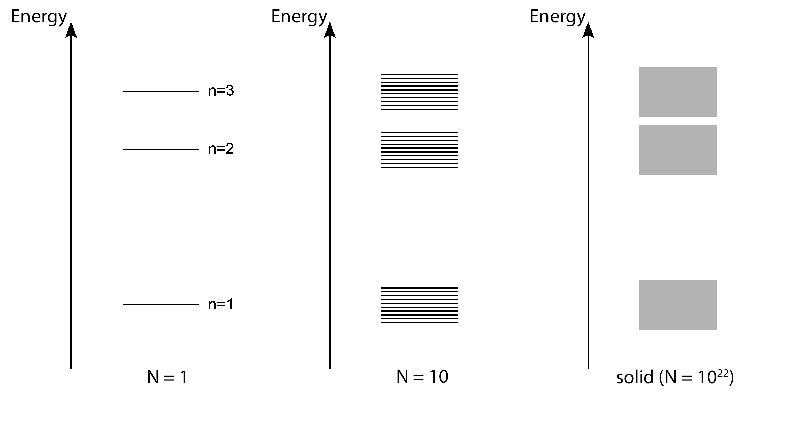
\includegraphics[width=1\linewidth]{chap1/fig/band_theory.pdf}
    \caption{\textbf{Energy levels of a set of N atoms.} As N increase the spacing between two successive levels tends to zero and eventually form a continuous band of energy.}
    \label{fig:band_theory}
\end{figure}

\subsection{Band structure of semiconductors}

Finding the exact band structure of a material can be done by solving the Schrodinger equation for an electron in periodic potential.
 The Bloch theorem states that the wave function of such an electron can be written as a plane wave modulated by a periodic function. The periodic function is then expanded in a Fourier series and the Schrodinger equation is solved for each Fourier component. 
 The exact band structure can be rather complicated but a simplified version can be obtained by considering the effective mass approximation \cite{kittel_introduction_2005}. In this picture, the dispersion relation of the electron in the material is typically represented in \autoref{fig:Direct_gap_disp}.
In this case the minimum of the conduction band and the maximum of the valence band are located at the same point in the Brillouin zone. The material is then said to have a direct band gap.
\begin{figure}[h]
    \centering
    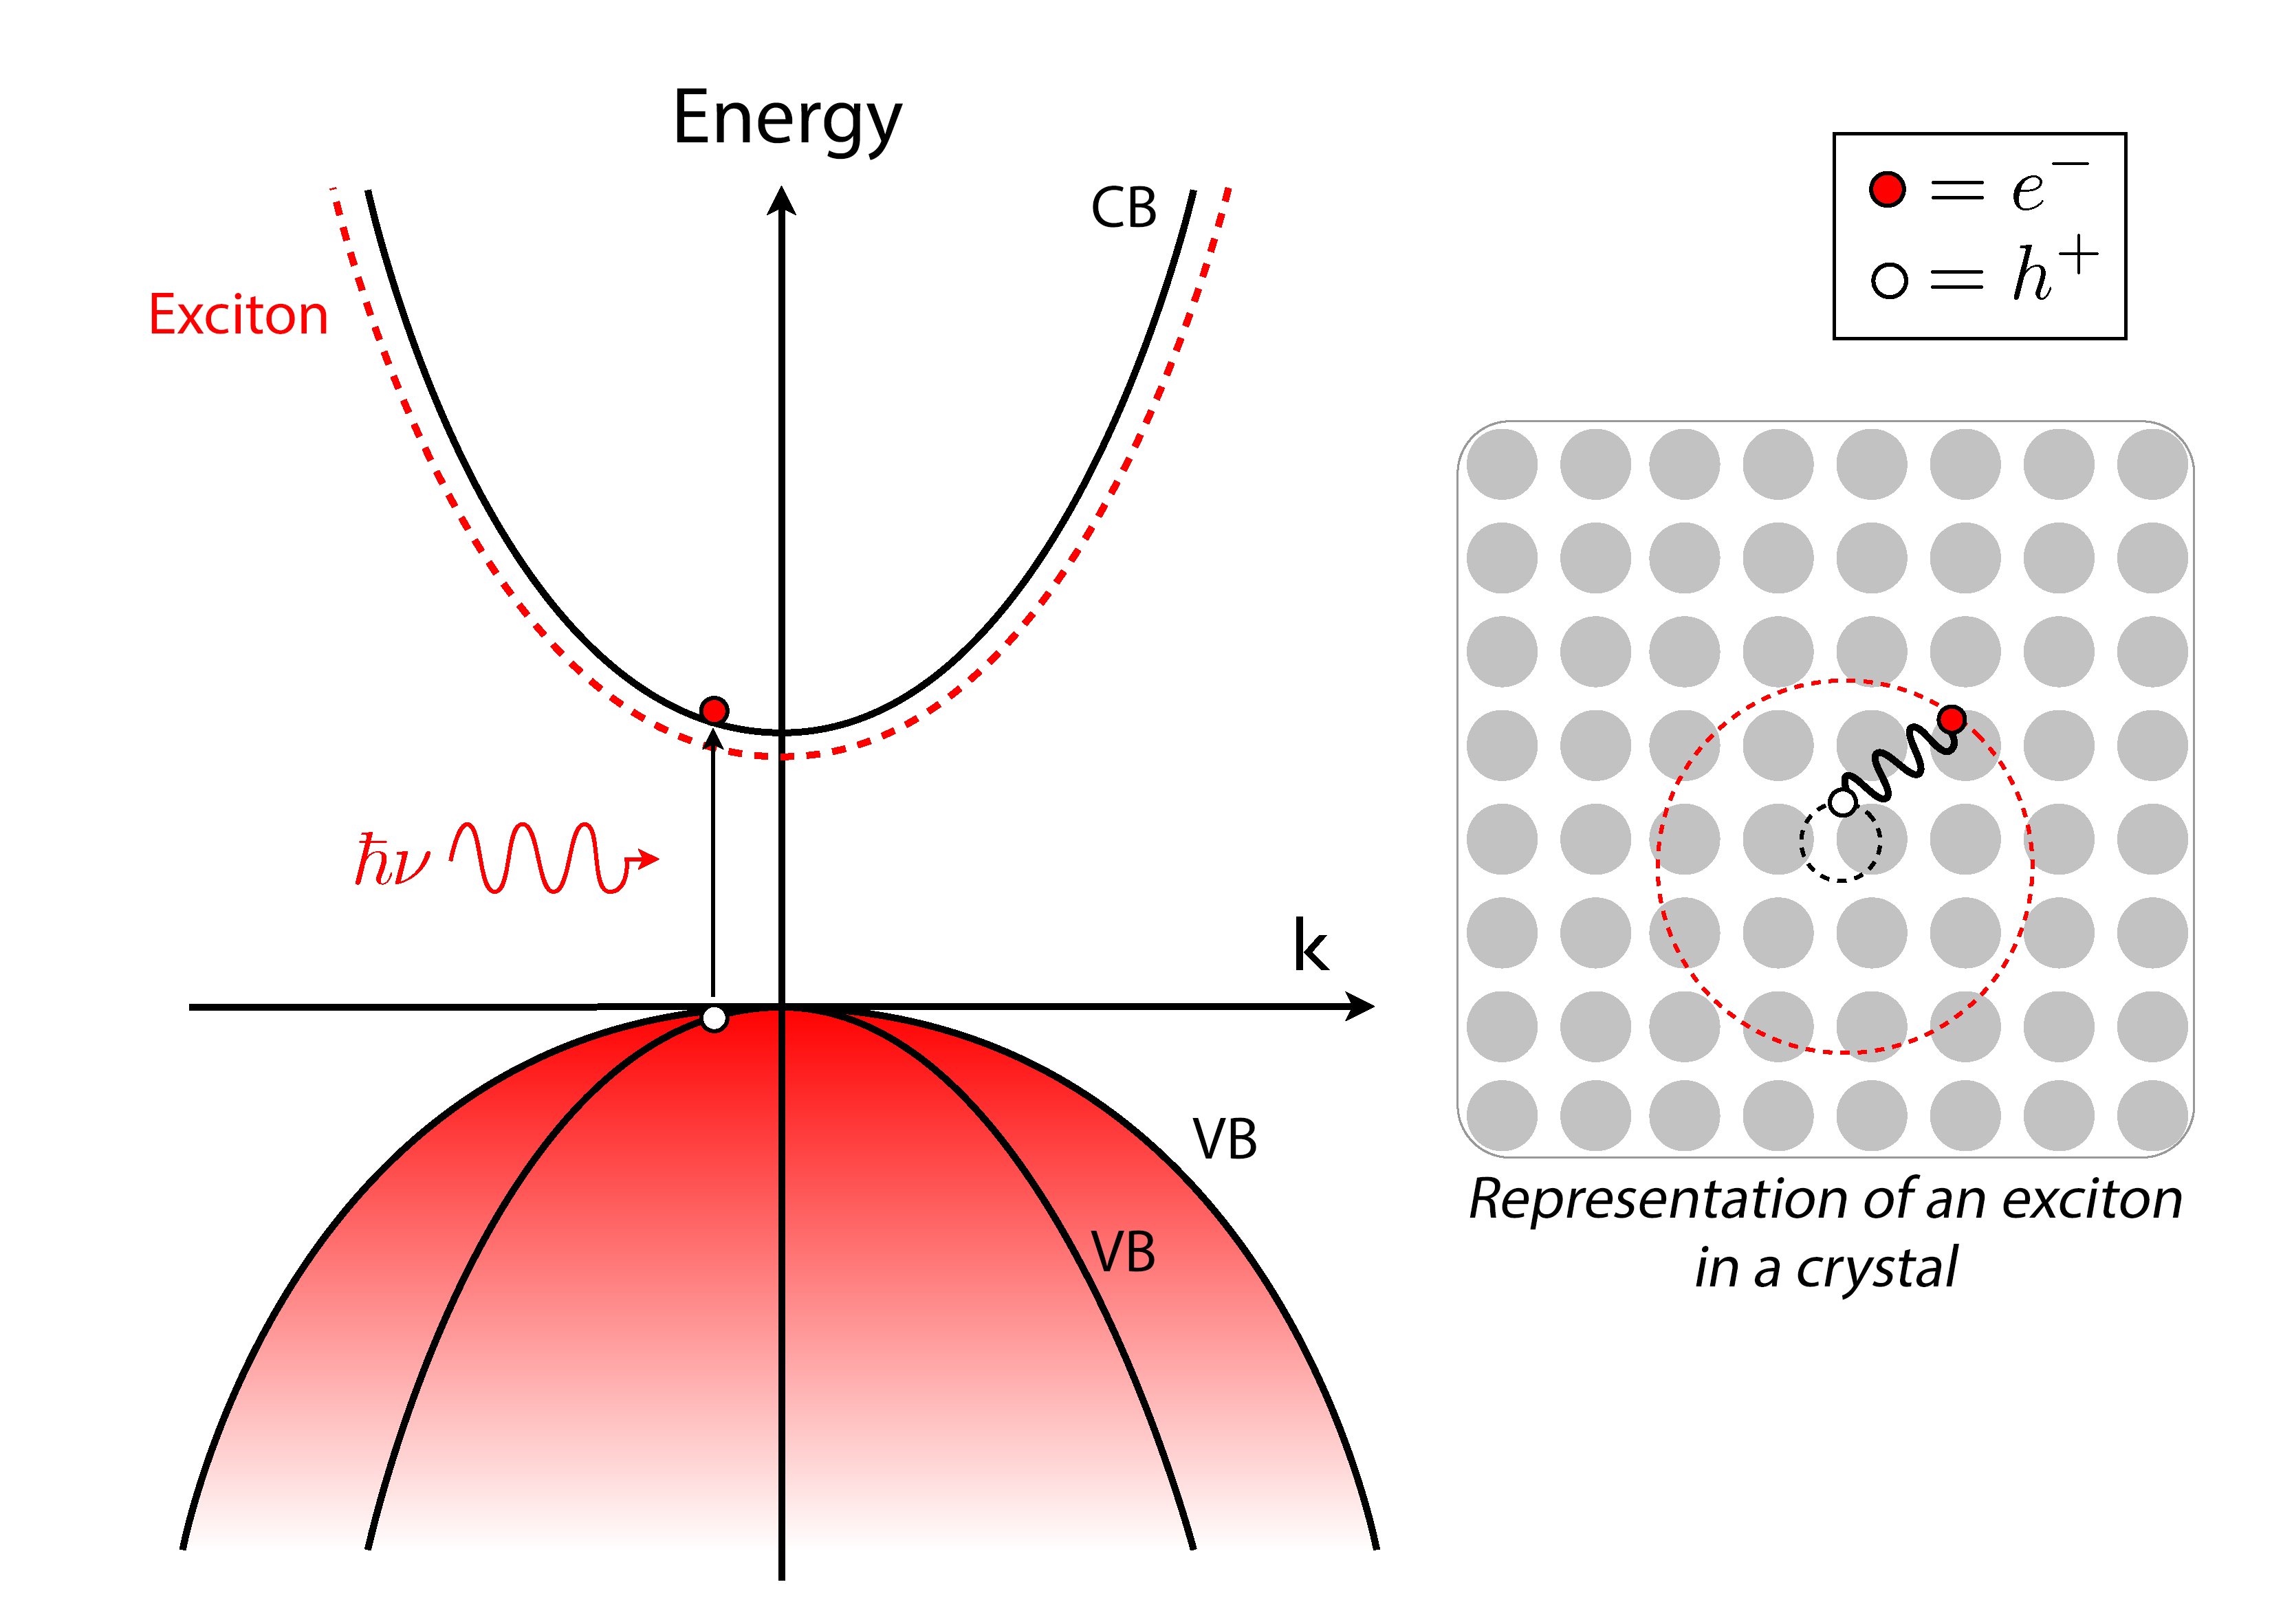
\includegraphics[width=0.8\linewidth]{chap1/fig/DirectGapDisp.png}
    \caption{\textbf{Band structure of a direct gap semiconductor.} The black solid line represent the conduction and valence band in a bulk semiconductor. The red dashed lines represent the dispersion relation of an exciton. The filling of the valence band by electrons is represented by the shaded red color.}
    \label{fig:Direct_gap_disp}
\end{figure}


\subsection{Excitons in bulk semiconductor}

As shown in \autoref{fig:Direct_gap_disp} shinning a photon whose energy exceed the gap energy can promote an electron from the valence band to the conduction band through absorption. 
The disappearance of the electron in the valence band can be described equivalently as the creation of a virtual particle of opposite charge called hole \cite{Combescot_cooper_excitons_2015}.
 If one scan shine a laser on a semiconductor and ramp up its frequency a narrow absorption peak is observed below the gap energy.  The presence of this peak originate from the coulombic interaction between the created electron and the hole creating a bound state of the material. In terms of energy it's as if the gap energy is reduced by the binding energy of the exciton and the electron lies in a virtual band below the conduction band as represented by the red dashed lines in \autoref{fig:Direct_gap_disp}.
 The exciton energy can then be written as : 

\begin{equation}
    E_{X} = E_g - E_b + \frac{\hbar^2 K^2}{2m_{X}}
\end{equation}

where $E_g$ is the gap energy, $E_b$ the binding energy,  $\hbar \vec{K}$ is the exciton momentum defined as the electron-hole pair center of mass momentum and $m_{X}$ the exciton effective mass which is the sum of the electron and hole effective mass.
Since $E_b$ is the interaction energy between a electron and a hole it is very similar to the Rydberg energy series of the hydrogen atom, the hole playing the role of the proton. As a consequence, the same electronic structure exist for the exciton : 1s, 2s, 2p, etc state can be observed in the absorption spectrum of the material.
However, the hole is quite different from the proton in the sense that it's actually a collective excitation of all the valence band electrons. Furthermore the exciton is a weakly bound state as the binding energy is typically a few meV. In GaAs or AlGaAs heterostructures which are the materials used in the present work $E_b$ is around 4 meV due to their high dielectric constant $\epsilon_r \sim 12$.
In these kind of samples, excitonic resonances can only be observed at cryogenic temperatures since the binding needs to exceeds the thermal energy $k_B T$ in order to survive the thermal fluctuations. For the above mentionned structures we obtain the condition $T<10$ K for excitons stability.
Another important exciton characteristic is their huge Bohr Radius $a_X= \frac{\epsilon_r \hbar^2}{m_X e^2}= 11.6 \ \mathrm{nm}$ in GaAs which  is much larger then the typical size of a unit crystalline cell $a_0 = 5.65 \SI{1}{\angstrom}$. This means that the exciton wavefunction is delocalized over many unit cells. Such excitons, are called Wannier-Mott and constrast with Frenkel excitons which are localized on a single unit cell and are typically found in organic materials.
 \bigskip\noindent

\subsection{A few words about exciton scattering}
As excitons are made of an electron and a hole bound by Coulombic interactions they undergo dipolar interactions.
 Since these interactions are precisely what will latter turn microcavity photons into an interacting quantum fluid, let us have a few words about the main scattering processes that can occur among the different electrons in the semiconductor. 
\bigskip

\begin{figure}[h]
    \centering
    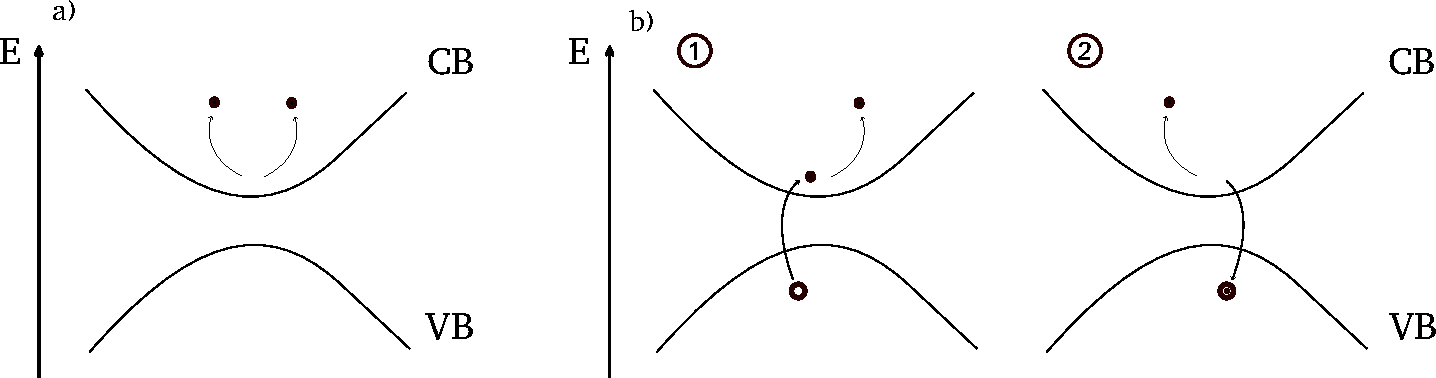
\includegraphics[width=1\linewidth]{chap1/fig/intra-inter-band-processes.pdf}
    \caption{\textbf{Drawing representing the scattering between two conduction band electrons.} a) Direct intraband scattering. Filled black dots represent conduction band electrons. b) Two steps scattering involving an electron-hole exchange or creation an annihilation of an exciton, referred as interband scattering.
    The empty black circle represent a valence band hole while the same circle with a small black dot inside stands for a valence band hole filled with an electron which is equivalent to a valence electron. a) and b) share the same
     final state which is a full valence band and two scattered conduction band electrons. Drawing inspired from \cite{Combescot_cooper_excitons_2015}.}
    \label{fig:inter-intra-scat}
\end{figure}


\textbf{Intraband scattering :}
to start with let's consider the direct scattering between two conduction band electrons as presented in \autoref{fig:inter-intra-scat} a). This simple process is referred as intraband scattering since each electron stays in its own band. In the small momentum limit $\mathrm{\textbf{q}}\to 0$ it yields a potential of the form:

\begin{equation}
    V_{\textbf{q}} \simeq \dfrac{4\pi e^2}{L^3 q^2}
\end{equation}
 
\noindent in a sample of size L. This form of potential holds also for the scattering between two valence electrons or between a valence and a conduction band electron that stay in their respective bands.

\bigskip

\textbf{Interband scattering :}
processes in which one or two electrons change band are also possible and are referred as interband scattering. In the case of a single 
interband jump the potential reads $(\frac{q}{\kappa})V_{\textbf{q}}= \dfrac{4\pi e^2}{L^3 q \kappa}$ where $\kappa$ is a dimensionnal factor that depends on the material. It then behaves as $1/q$. When both electrons change band the potential is then $(\frac{q}{\kappa})^2V_{\textbf{q}}$ proportionnal to $q^0$
and thus remaining finite when $q\to 0$. Remarkably, in both the single and two interband jump scenarios, the number of electrons in each band changes by one and two, respectively, making these transitions less likely to occur compared to number-conserving processes.

\bigskip
Indeed, in second order perturbation theory the transition amplitude between an initial state $\ket{i}$ and a final state $\ket{f}$ may be written as :

\begin{equation}
    \Gamma_{i\to f}^{(2)} = \dfrac{2\pi}{\hbar} \bigg \vert \sum_{m} \dfrac{\bra{f}V_q\ket{m}\bra{m}V_q\ket{i}}{E_i - E_m}\bigg \vert^2 \delta(E_f - E_i)
    \label{eq:transition_amplitude}
\end{equation}

\noindent Whenever an electron undergo a band jump the energy cost is of the order of the band gap $E_f - E_i \simeq E_g$. As a consequence the corresponding transition amplitude gets reduced by a factor $\frac{1}{E_g}$ and appears to be negligible.
 However a direct intraband scattering can happen in several interband jumps that will dress the direct Coulomb scattering as shown in \autoref{fig:inter-intra-scat} b) for the case of two jumps. When summing over all possible intermediate state as is \eqref{eq:transition_amplitude} we end up with the same potential as the direct intraband scattering but reduced by dielectric constant factor $\epsilon_{sc}$ that depend on the material.

 
\bigskip




To clarify this idea let us now consider the scattering between a conduction and a valence band electron. 
The same scattering process can also occur in two steps. First, a conduction band electron is scattered in its band while a valence band electron is promoted to the conduction band. Since an electron changes band it brings a potential $V_q(q/\kappa)$. Secondly, 
 the excited electron goes back to the valence band while a valence band electron is scattered in its band yielding again a potential $V_q(q/\kappa)$. This two steps interaction end up with the same initial and final states than direct intraband scattering and the number of electrons in each band is conserved.  
In terms of energy, the two scatterings behaving as $1/q$ potentials the overall potential behaves also as $1/q^2$ but with an additionnal $1/E_{g}$ factor coming from the intermediate interband jumps. More specifically the two steps contribution is : $\left( 4\pi e^2/L^3q^2 \right)\left[ (e^2/L^3\kappa^2)/E_{g}\right]$.  

\bigskip
It is also possible to make it a three steps scattering by adding an intermediate interband exchange after the first step : the previously excited conduction band electron returns to the valence band while a valence band electron is promoted to the conduction band. 
Moe explicitly the process is as follows : 

\begin{itemize}
    \item \textbf{Step 1 :} a valence band electron is promoted to the conduction band while a conduction bandis scattered in its band. The potential reads $V_q(q/\kappa) \propto \frac{1}{q}$ and the energy cost is of the order of $E_g$.
    \item \textbf{Step 2 :} the previously excited conduction band electron returns to the valence band while another valence band electron is excited to the conduction band. The potential read $V_q(q/\kappa)^2 \propto q$ and the energy cost is of the order of $2E_g$.
    \item \textbf{Step 3 :} the excited electron goes back to the valence band while a valence band electron is scattered in its band. The potential read again $V_q(q/\kappa) \propto \frac{1}{q}$ and the energy cost is of the order of $E_g$.
\end{itemize}

\noindent The total energy budget is then : $\left( 4\pi e^2/L^3q^2 \right)\left[ (e^2/L^3\kappa^2)/E_{g}\right]^2$. Remarkably, one might expect the overall potential to scale as $1/E_g^3$  since each step requires at least one electron to change band. However, the structure of perturbation theory ensures that the total energy denominator accounts for the number of coupled interband transitions, rather than treating each step independently. 
Step 2 effectively "couples" the transitions in such a way that two energy denominators are introduced, rather than three independent ones, which explains the 
$1/E_g^2$ dependence. This coupling reflects the fact that intermediate states are shared between adjacent steps in the perturbative sequence.
\bigskip 


\begin{figure}[h]
    \centering
    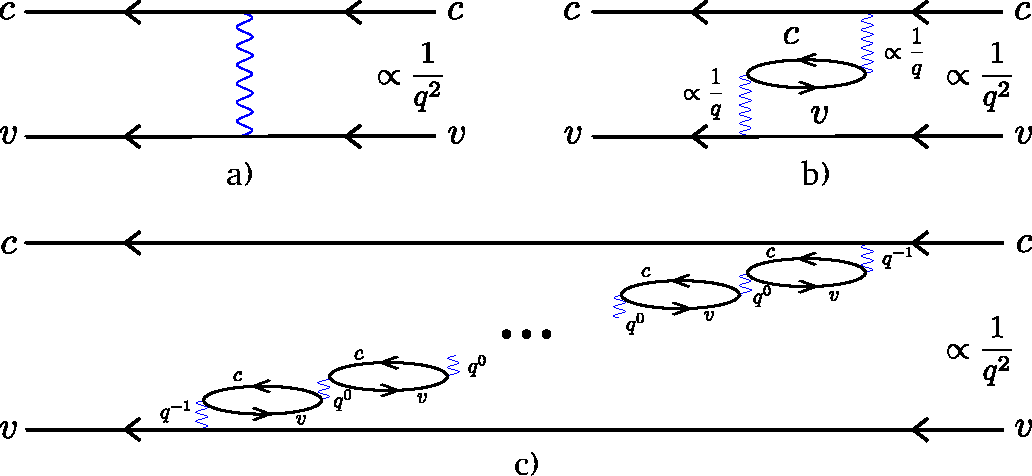
\includegraphics[width=1\linewidth]{chap1/fig/intra_band_dressed_bubbles.pdf}
    \caption{\textbf{Feynman diagrams representing an intraband scattering between a conduction and a valence band electron.} a) Direct intraband scattering. The blue wavy lines represent the Coulomb interaction that make the electrons to change states. b) Two steps scattering involving an intermediate interband exchange that is represented by the bubble in the middle.
    c) Multiple steps scattering involving several interband exchanges represented by the numerous bubbles.
    Drawing inspired from \cite{Combescot_cooper_excitons_2015}.}
    \label{fig:intra_bubbles}
\end{figure}

Finally, the number of intermediate states can be arbitrarily increased by adding 'bubbles' of exchange interaction, as illustrated in the Feynman diagram in \autoref{fig:intra_bubbles} b). Each pair of adjacent bubbles represents an interband interaction similar to the one described in Step 2 above. While it conserves the number of electrons in each band, it involves two interband jumps. 
The interaction between two bubbles is then $\propto q^0$ and is finite in the small momentum limit.
By summing the contributions of processes with all possible numbers of bubbles, we obtain an effective Coulomb potential:

\begin{equation}
    V_q = \dfrac{4\pi e^2}{L^3q^2\epsilon_{sc}}
\end{equation}

where $\epsilon_{sc}$ is a dielectric constant mainly stemming from the infinite sum over the number of bubbles.






\noindent\textbf{Exciton-photon interaction :} Experimentally excitons appears as narrow lines in the absorption spectrum of the material as excitons are bound states that are very well coupled to photons. 
The interaction at stake when a photon is absorbed by the material an thus mediating the creation of an exciton can be described by a simple electron-photon Hamiltonian which in the electric dipole approximation reads :

\begin{equation}
    \Ham_{dip} = -e \dfrac{\vec{p_e} \cdot \vec{A}}{m^*_e},
\end{equation}

with $\vec{p_e}$ the momentum operator of the electron and $\vec{A}$ the potential vector of the electromagnetic field. Before going further let us have a look at what the symetries of this Hamiltonian imply based on the Noether theorem.

\begin{itemize}
    \item \textbf{Total momentum conservation :}  translational invariance of the system implies that the total momentum of the system is conserved. The absorption of a photon with momentum 
    $\hbar \vec{k_c}$ will create an exciton with the same momentum.
    \item  \textbf{Total angular momentum conservation :} rotational invariance of the system implies that the total angular momentum of the system is conserved along the interaction.
\end{itemize}

The second point raises the question of the possible values that the exciton angular momentum can assume. To answer this question we need to get back to its 
microscopic constitutive particles : a conduction band electron and a hole in the valence band. In usual semiconductors a conduction band electron has an orbital angular momentum ($L=0 , L_z=0$) while a valence band electron yields ($L=1 , L_z=(+1,0,-1)$) (see \cite{Combescot_cooper_excitons_2015}).
Since $J_z = J_z + S_z$ and the electron spin is $S_z = \pm 1/2$ we obtain for the valence band $J_z^{v} = (3/2, 1/2, -1/2, -3/2)$ and for the conduction band $J_z^{c} = \pm 1/2$. If we now move to the electron-hole picture the electron angular momentum remains unchanged $J_z^{e}=J_z^{c}= \pm 1/2$ while the hole angular momentum is the opposite of the valence band electron $J_z^{h} = -J_z^{v}=(3/2, 1/2, -1/2, -3/2)$.
 The exciton angular momentum is then $J_z = J_z^{e} + J_z^{h} = (-2,-1,0,1,2)$. We can thus distinguish \textbf{bright} excitons with $J_z = (-1,0,1)$ that couple to light with polarization $\pi , \sigma_+ , \sigma_-$ and \textbf{dark} excitons with $J_z = (-2,2)$ that do not couple to light. 

\textbf{Dark-bright exciton splitting : } 